% Created by tikzDevice version 0.6.2 on 2014-03-28 11:37:36
% !TEX encoding = UTF-8 Unicode
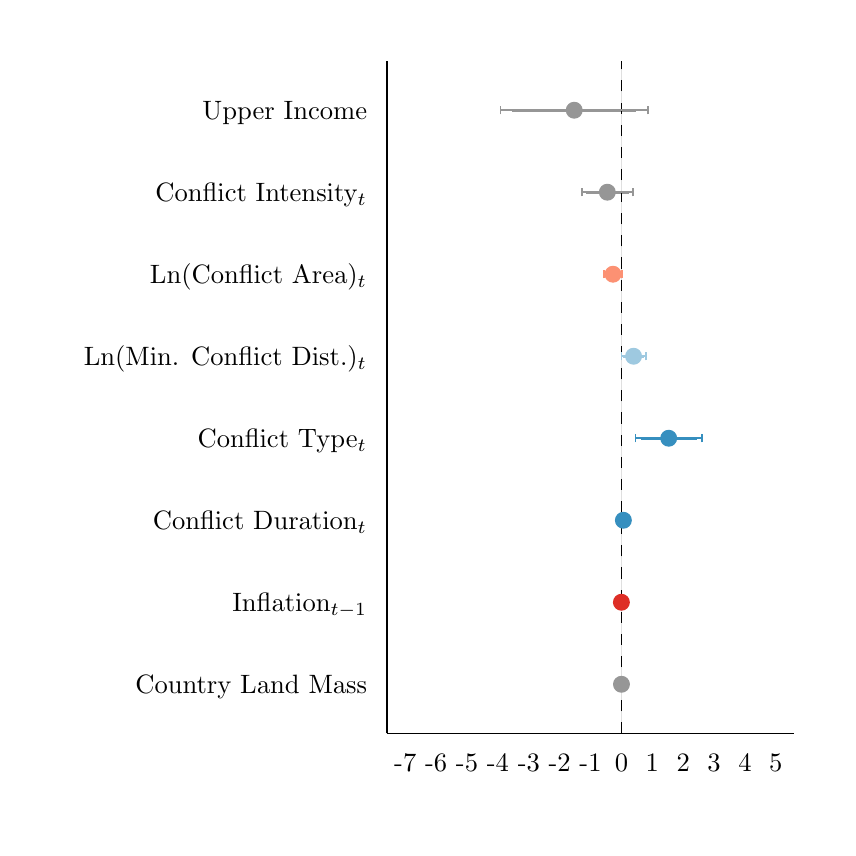
\begin{tikzpicture}[x=1pt,y=1pt]
\definecolor[named]{drawColor}{rgb}{0.00,0.00,0.00}
\definecolor[named]{fillColor}{rgb}{1.00,1.00,1.00}
\fill[color=fillColor,fill opacity=0.00,] (0,0) rectangle (289.08,289.08);
\begin{scope}
\path[clip] (  0.00,  0.00) rectangle (289.08,289.08);
\end{scope}
\begin{scope}
\path[clip] (  0.00,  0.00) rectangle (289.08,289.08);
\end{scope}
\begin{scope}
\path[clip] (  0.00,  0.00) rectangle (289.08,289.08);
\definecolor[named]{drawColor}{rgb}{1.00,1.00,1.00}
\definecolor[named]{fillColor}{rgb}{1.00,1.00,1.00}

\draw[color=drawColor,line width= 0.6pt,line cap=round,line join=round,fill=fillColor,] ( -0.00,  0.00) rectangle (289.08,289.08);
\end{scope}
\begin{scope}
\path[clip] (  0.00,  0.00) rectangle (289.08,289.08);
\end{scope}
\begin{scope}
\path[clip] (  0.00,  0.00) rectangle (289.08,289.08);
\end{scope}
\begin{scope}
\path[clip] (  0.00,  0.00) rectangle (289.08,289.08);
\end{scope}
\begin{scope}
\path[clip] (129.77, 34.03) rectangle (277.03,277.03);
\definecolor[named]{fillColor}{rgb}{1.00,1.00,1.00}

\draw[fill=fillColor,draw opacity=0.00,] (129.77, 34.03) rectangle (277.03,277.03);
\definecolor[named]{drawColor}{rgb}{0.59,0.59,0.59}
\definecolor[named]{fillColor}{rgb}{0.59,0.59,0.59}

\draw[color=drawColor,line width= 0.3pt,line join=round,fill=fillColor,fill opacity=0.30,draw opacity=0.30,] (214.56, 51.82) -- (214.56, 51.82);
\definecolor[named]{drawColor}{rgb}{0.87,0.18,0.15}
\definecolor[named]{fillColor}{rgb}{0.87,0.18,0.15}

\draw[color=drawColor,line width= 0.3pt,line join=round,fill=fillColor,fill opacity=0.30,draw opacity=0.30,] (214.53, 81.45) -- (214.55, 81.45);
\definecolor[named]{drawColor}{rgb}{0.21,0.56,0.75}
\definecolor[named]{fillColor}{rgb}{0.21,0.56,0.75}

\draw[color=drawColor,line width= 0.3pt,line join=round,fill=fillColor,fill opacity=0.30,draw opacity=0.30,] (214.90,111.08) -- (215.62,111.08);

\draw[color=drawColor,line width= 0.3pt,line join=round,fill=fillColor,fill opacity=0.30,draw opacity=0.30,] (219.64,140.72) -- (243.62,140.72);
\definecolor[named]{drawColor}{rgb}{0.62,0.79,0.88}
\definecolor[named]{fillColor}{rgb}{0.62,0.79,0.88}

\draw[color=drawColor,line width= 0.3pt,line join=round,fill=fillColor,fill opacity=0.30,draw opacity=0.30,] (214.53,170.35) -- (223.35,170.35);
\definecolor[named]{drawColor}{rgb}{0.99,0.57,0.45}
\definecolor[named]{fillColor}{rgb}{0.99,0.57,0.45}

\draw[color=drawColor,line width= 0.3pt,line join=round,fill=fillColor,fill opacity=0.30,draw opacity=0.30,] (208.31,199.99) -- (214.71,199.99);
\definecolor[named]{drawColor}{rgb}{0.59,0.59,0.59}
\definecolor[named]{fillColor}{rgb}{0.59,0.59,0.59}

\draw[color=drawColor,line width= 0.3pt,line join=round,fill=fillColor,fill opacity=0.30,draw opacity=0.30,] (200.24,229.62) -- (218.68,229.62);

\draw[color=drawColor,line width= 0.3pt,line join=round,fill=fillColor,fill opacity=0.30,draw opacity=0.30,] (170.81,259.25) -- (224.20,259.25);
\definecolor[named]{drawColor}{rgb}{0.59,0.59,0.59}
\definecolor[named]{fillColor}{rgb}{0.59,0.59,0.59}

\draw[color=drawColor,line width= 1.1pt,line join=round,fill=fillColor,] (214.56, 51.82) -- (214.56, 51.82);
\definecolor[named]{drawColor}{rgb}{0.87,0.18,0.15}
\definecolor[named]{fillColor}{rgb}{0.87,0.18,0.15}

\draw[color=drawColor,line width= 1.1pt,line join=round,fill=fillColor,] (214.53, 81.45) -- (214.55, 81.45);
\definecolor[named]{drawColor}{rgb}{0.21,0.56,0.75}
\definecolor[named]{fillColor}{rgb}{0.21,0.56,0.75}

\draw[color=drawColor,line width= 1.1pt,line join=round,fill=fillColor,] (214.96,111.08) -- (215.57,111.08);

\draw[color=drawColor,line width= 1.1pt,line join=round,fill=fillColor,] (221.57,140.72) -- (241.69,140.72);
\definecolor[named]{drawColor}{rgb}{0.62,0.79,0.88}
\definecolor[named]{fillColor}{rgb}{0.62,0.79,0.88}

\draw[color=drawColor,line width= 1.1pt,line join=round,fill=fillColor,] (215.24,170.35) -- (222.64,170.35);
\definecolor[named]{drawColor}{rgb}{0.99,0.57,0.45}
\definecolor[named]{fillColor}{rgb}{0.99,0.57,0.45}

\draw[color=drawColor,line width= 1.1pt,line join=round,fill=fillColor,] (208.82,199.99) -- (214.20,199.99);
\definecolor[named]{drawColor}{rgb}{0.59,0.59,0.59}
\definecolor[named]{fillColor}{rgb}{0.59,0.59,0.59}

\draw[color=drawColor,line width= 1.1pt,line join=round,fill=fillColor,] (201.72,229.62) -- (217.20,229.62);

\draw[color=drawColor,line width= 1.1pt,line join=round,fill=fillColor,] (175.10,259.25) -- (219.90,259.25);
\definecolor[named]{drawColor}{rgb}{0.00,0.00,0.00}
\definecolor[named]{fillColor}{rgb}{0.00,0.00,0.00}

\draw[color=drawColor,line width= 0.6pt,dash pattern=on 4pt off 4pt ,line join=round,fill=fillColor,] (214.56, 34.03) -- (214.56,277.03);
\definecolor[named]{drawColor}{rgb}{0.59,0.59,0.59}
\definecolor[named]{fillColor}{rgb}{0.59,0.59,0.59}

\draw[color=drawColor,line cap=round,line join=round,fill=fillColor,] (197.50,259.25) circle (  2.85);

\draw[color=drawColor,line cap=round,line join=round,fill=fillColor,] (209.46,229.62) circle (  2.85);
\definecolor[named]{drawColor}{rgb}{0.99,0.57,0.45}
\definecolor[named]{fillColor}{rgb}{0.99,0.57,0.45}

\draw[color=drawColor,line cap=round,line join=round,fill=fillColor,] (211.51,199.99) circle (  2.85);
\definecolor[named]{drawColor}{rgb}{0.62,0.79,0.88}
\definecolor[named]{fillColor}{rgb}{0.62,0.79,0.88}

\draw[color=drawColor,line cap=round,line join=round,fill=fillColor,] (218.94,170.35) circle (  2.85);
\definecolor[named]{drawColor}{rgb}{0.21,0.56,0.75}
\definecolor[named]{fillColor}{rgb}{0.21,0.56,0.75}

\draw[color=drawColor,line cap=round,line join=round,fill=fillColor,] (231.63,140.72) circle (  2.85);

\draw[color=drawColor,line cap=round,line join=round,fill=fillColor,] (215.26,111.08) circle (  2.85);
\definecolor[named]{drawColor}{rgb}{0.87,0.18,0.15}
\definecolor[named]{fillColor}{rgb}{0.87,0.18,0.15}

\draw[color=drawColor,line cap=round,line join=round,fill=fillColor,] (214.54, 81.45) circle (  2.85);
\definecolor[named]{drawColor}{rgb}{0.59,0.59,0.59}
\definecolor[named]{fillColor}{rgb}{0.59,0.59,0.59}

\draw[color=drawColor,line cap=round,line join=round,fill=fillColor,] (214.56, 51.82) circle (  2.85);

\draw[color=drawColor,line width= 0.6pt,line join=round,] (214.56, 50.33) --
	(214.56, 53.30);

\draw[color=drawColor,line width= 0.6pt,line join=round,] (214.56, 51.82) --
	(214.56, 51.82);

\draw[color=drawColor,line width= 0.6pt,line join=round,] (214.56, 50.33) --
	(214.56, 53.30);
\definecolor[named]{drawColor}{rgb}{0.87,0.18,0.15}
\definecolor[named]{fillColor}{rgb}{0.87,0.18,0.15}

\draw[color=drawColor,line width= 0.6pt,line join=round,] (214.55, 79.97) --
	(214.55, 82.93);

\draw[color=drawColor,line width= 0.6pt,line join=round,] (214.55, 81.45) --
	(214.53, 81.45);

\draw[color=drawColor,line width= 0.6pt,line join=round,] (214.53, 79.97) --
	(214.53, 82.93);
\definecolor[named]{drawColor}{rgb}{0.21,0.56,0.75}
\definecolor[named]{fillColor}{rgb}{0.21,0.56,0.75}

\draw[color=drawColor,line width= 0.6pt,line join=round,] (215.62,109.60) --
	(215.62,112.57);

\draw[color=drawColor,line width= 0.6pt,line join=round,] (215.62,111.08) --
	(214.90,111.08);

\draw[color=drawColor,line width= 0.6pt,line join=round,] (214.90,109.60) --
	(214.90,112.57);

\draw[color=drawColor,line width= 0.6pt,line join=round,] (243.62,139.24) --
	(243.62,142.20);

\draw[color=drawColor,line width= 0.6pt,line join=round,] (243.62,140.72) --
	(219.64,140.72);

\draw[color=drawColor,line width= 0.6pt,line join=round,] (219.64,139.24) --
	(219.64,142.20);
\definecolor[named]{drawColor}{rgb}{0.62,0.79,0.88}
\definecolor[named]{fillColor}{rgb}{0.62,0.79,0.88}

\draw[color=drawColor,line width= 0.6pt,line join=round,] (223.35,168.87) --
	(223.35,171.83);

\draw[color=drawColor,line width= 0.6pt,line join=round,] (223.35,170.35) --
	(214.53,170.35);

\draw[color=drawColor,line width= 0.6pt,line join=round,] (214.53,168.87) --
	(214.53,171.83);
\definecolor[named]{drawColor}{rgb}{0.99,0.57,0.45}
\definecolor[named]{fillColor}{rgb}{0.99,0.57,0.45}

\draw[color=drawColor,line width= 0.6pt,line join=round,] (214.71,198.50) --
	(214.71,201.47);

\draw[color=drawColor,line width= 0.6pt,line join=round,] (214.71,199.99) --
	(208.31,199.99);

\draw[color=drawColor,line width= 0.6pt,line join=round,] (208.31,198.50) --
	(208.31,201.47);
\definecolor[named]{drawColor}{rgb}{0.59,0.59,0.59}
\definecolor[named]{fillColor}{rgb}{0.59,0.59,0.59}

\draw[color=drawColor,line width= 0.6pt,line join=round,] (218.68,228.14) --
	(218.68,231.10);

\draw[color=drawColor,line width= 0.6pt,line join=round,] (218.68,229.62) --
	(200.24,229.62);

\draw[color=drawColor,line width= 0.6pt,line join=round,] (200.24,228.14) --
	(200.24,231.10);

\draw[color=drawColor,line width= 0.6pt,line join=round,] (224.20,257.77) --
	(224.20,260.74);

\draw[color=drawColor,line width= 0.6pt,line join=round,] (224.20,259.25) --
	(170.81,259.25);

\draw[color=drawColor,line width= 0.6pt,line join=round,] (170.81,257.77) --
	(170.81,260.74);
\end{scope}
\begin{scope}
\path[clip] (  0.00,  0.00) rectangle (289.08,289.08);
\end{scope}
\begin{scope}
\path[clip] (  0.00,  0.00) rectangle (289.08,289.08);
\definecolor[named]{drawColor}{rgb}{0.00,0.00,0.00}

\draw[color=drawColor,line width= 0.6pt,line join=round,fill opacity=0.00,] (129.77, 34.03) --
	(129.77,277.03);
\end{scope}
\begin{scope}
\path[clip] (  0.00,  0.00) rectangle (289.08,289.08);
\definecolor[named]{drawColor}{rgb}{0.00,0.00,0.00}

\node[color=drawColor,anchor=base east,inner sep=0pt, outer sep=0pt, scale=  0.96] at (122.65, 48.51) {Country Land Mass};

\node[color=drawColor,anchor=base east,inner sep=0pt, outer sep=0pt, scale=  0.96] at (122.65, 78.14) {Inflation$_{t-1}$};

\node[color=drawColor,anchor=base east,inner sep=0pt, outer sep=0pt, scale=  0.96] at (122.65,107.78) {Conflict Duration$_{t}$};

\node[color=drawColor,anchor=base east,inner sep=0pt, outer sep=0pt, scale=  0.96] at (122.65,137.41) {Conflict Type$_{t}$};

\node[color=drawColor,anchor=base east,inner sep=0pt, outer sep=0pt, scale=  0.96] at (122.65,167.05) {Ln(Min. Conflict Dist.)$_{t}$};

\node[color=drawColor,anchor=base east,inner sep=0pt, outer sep=0pt, scale=  0.96] at (122.65,196.68) {Ln(Conflict Area)$_{t}$};

\node[color=drawColor,anchor=base east,inner sep=0pt, outer sep=0pt, scale=  0.96] at (122.65,226.31) {Conflict Intensity$_{t}$};

\node[color=drawColor,anchor=base east,inner sep=0pt, outer sep=0pt, scale=  0.96] at (122.65,255.95) {Upper Income};
\end{scope}
\begin{scope}
\path[clip] (  0.00,  0.00) rectangle (289.08,289.08);
\end{scope}
\begin{scope}
\path[clip] (  0.00,  0.00) rectangle (289.08,289.08);
\end{scope}
\begin{scope}
\path[clip] (  0.00,  0.00) rectangle (289.08,289.08);
\end{scope}
\begin{scope}
\path[clip] (  0.00,  0.00) rectangle (289.08,289.08);
\end{scope}
\begin{scope}
\path[clip] (  0.00,  0.00) rectangle (289.08,289.08);
\end{scope}
\begin{scope}
\path[clip] (  0.00,  0.00) rectangle (289.08,289.08);
\end{scope}
\begin{scope}
\path[clip] (  0.00,  0.00) rectangle (289.08,289.08);
\definecolor[named]{drawColor}{rgb}{0.00,0.00,0.00}

\draw[color=drawColor,line width= 0.6pt,line join=round,fill opacity=0.00,] (129.77, 34.03) --
	(277.03, 34.03);
\end{scope}
\begin{scope}
\path[clip] (  0.00,  0.00) rectangle (289.08,289.08);
\end{scope}
\begin{scope}
\path[clip] (  0.00,  0.00) rectangle (289.08,289.08);
\end{scope}
\begin{scope}
\path[clip] (  0.00,  0.00) rectangle (289.08,289.08);
\definecolor[named]{drawColor}{rgb}{0.00,0.00,0.00}

\node[color=drawColor,anchor=base,inner sep=0pt, outer sep=0pt, scale=  0.96] at (136.46, 20.31) {-7};

\node[color=drawColor,anchor=base,inner sep=0pt, outer sep=0pt, scale=  0.96] at (147.62, 20.31) {-6};

\node[color=drawColor,anchor=base,inner sep=0pt, outer sep=0pt, scale=  0.96] at (158.77, 20.31) {-5};

\node[color=drawColor,anchor=base,inner sep=0pt, outer sep=0pt, scale=  0.96] at (169.93, 20.31) {-4};

\node[color=drawColor,anchor=base,inner sep=0pt, outer sep=0pt, scale=  0.96] at (181.09, 20.31) {-3};

\node[color=drawColor,anchor=base,inner sep=0pt, outer sep=0pt, scale=  0.96] at (192.24, 20.31) {-2};

\node[color=drawColor,anchor=base,inner sep=0pt, outer sep=0pt, scale=  0.96] at (203.40, 20.31) {-1};

\node[color=drawColor,anchor=base,inner sep=0pt, outer sep=0pt, scale=  0.96] at (214.56, 20.31) {0};

\node[color=drawColor,anchor=base,inner sep=0pt, outer sep=0pt, scale=  0.96] at (225.71, 20.31) {1};

\node[color=drawColor,anchor=base,inner sep=0pt, outer sep=0pt, scale=  0.96] at (236.87, 20.31) {2};

\node[color=drawColor,anchor=base,inner sep=0pt, outer sep=0pt, scale=  0.96] at (248.03, 20.31) {3};

\node[color=drawColor,anchor=base,inner sep=0pt, outer sep=0pt, scale=  0.96] at (259.18, 20.31) {4};

\node[color=drawColor,anchor=base,inner sep=0pt, outer sep=0pt, scale=  0.96] at (270.34, 20.31) {5};
\end{scope}
\begin{scope}
\path[clip] (  0.00,  0.00) rectangle (289.08,289.08);
\end{scope}
\begin{scope}
\path[clip] (  0.00,  0.00) rectangle (289.08,289.08);
\end{scope}
\begin{scope}
\path[clip] (  0.00,  0.00) rectangle (289.08,289.08);
\end{scope}
\begin{scope}
\path[clip] (  0.00,  0.00) rectangle (289.08,289.08);
\end{scope}
\begin{scope}
\path[clip] (  0.00,  0.00) rectangle (289.08,289.08);
\end{scope}
\begin{scope}
\path[clip] (  0.00,  0.00) rectangle (289.08,289.08);
\end{scope}
\begin{scope}
\path[clip] (  0.00,  0.00) rectangle (289.08,289.08);
\end{scope}
\begin{scope}
\path[clip] (  0.00,  0.00) rectangle (289.08,289.08);
\end{scope}
\begin{scope}
\path[clip] (  0.00,  0.00) rectangle (289.08,289.08);
\end{scope}
\begin{scope}
\path[clip] (  0.00,  0.00) rectangle (289.08,289.08);
\end{scope}
\begin{scope}
\path[clip] (  0.00,  0.00) rectangle (289.08,289.08);
\end{scope}
\end{tikzpicture}
